\documentclass{beamer}

\mode<presentation>
{
  \usetheme{default}      % or try Darmstadt, Madrid, Warsaw, ...
  \usecolortheme{default} % or try albatross, beaver, crane, ...
  \usefonttheme{default}  % or try serif, structurebold, ...
  \setbeamertemplate{navigation symbols}{}
  \setbeamertemplate{caption}[numbered]
} 

\usepackage[english]{babel}
\usepackage[utf8]{inputenc}
\usepackage[T1]{fontenc}

\title[Your Short Title]{Combinatorial Analysis of Enigma Machine}
\author{Skylar Liang, Samie Amriui}
\date{May 6, 2020}

\begin{document}

\begin{frame}
  \titlepage
\end{frame}

% Uncomment these lines for an automatically generated outline.
\begin{frame}{Outline}
  \tableofcontents
\end{frame}

\section{Introduction}
\subsection{Background of Enigma Machine}
\begin{frame}{Background of Enigma Machine}

\begin{itemize}
   \item The Enigma Machine was invented by the German engineer Arthur Scherbius at the end of World War I in 1918.
   \item It is an encryption machine that looks like a typewriter.
   \item During World War II, Nazi German used the Enigma Machines to communicate.
\end{itemize}
\vskip 1cm
\begin{figure}
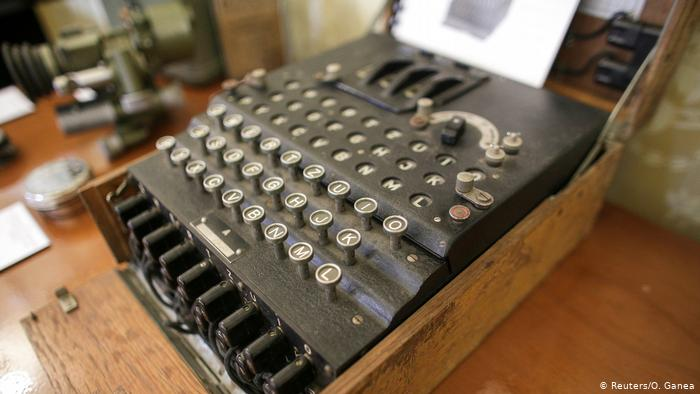
\includegraphics[scale=0.3]{Enigma_Machine.jpg}
\caption{An enigma machine used during WWII}
\end{figure}
% \begin{block}{Examples}
% Some examples of commonly used commands and features are included, to help you get started.
% \end{block}
\end{frame}

\subsection{Interest in the Enigma Machine}
\begin{frame}{Interest in the Enigma Machine}
The Enigma Machine was an outstanding innovation at that time in history.
\par Although the Enigma Machine was ultimately decrypted by Alan Turing, it proved to have immeasurable relevance to today’s development in technology since it introduced the concept of encryption through electrical and mechanical circuits.
    
\end{frame}
\section{Combinatorial theories in the Enigma Machine}

\subsection{Mechanism of Enigma Machine in the Military}

\begin{frame}{Mechanism of Enigma Machine in the Military}
The step by step process of an Enigma Machine:
\begin{itemize}
%\item Use \texttt{tabular} for basic tables --- see Table~\ref{tab:widgets}, for example.
\item During WWII, Nazi German operators of the enigma machine would choose three rotors from five possible choices that provide an alphabet order \cite{MLB}.
\item Standard machine: 3 rotors, each with 26 letters carved on.
\item Starting from right to left, when a letter is pressed, the current rotor rotates by 1
\item Once the current rotor reaches its "turnover" position, which is set by human, it kicks the next rotor to move.
\end{itemize}
\end{frame}

\begin{frame}{The plug-board}
During WWII, the Nazis also included another feature which is the plug board.
\begin{itemize}
    \item A board with 26 letters and 10 wires.
    \item Each wire will connect two letters together, and leave 6 letters untouched.
    \item Once connected with another letter, this letter's encryption method will be swapped with its pair. 
\end{itemize}
\begin{figure}
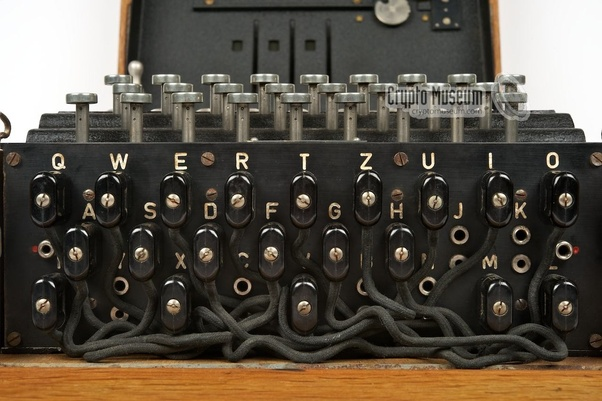
\includegraphics[scale=0.2]{plug board.jpeg}
\caption{The plug-board of an Enigma Machine}
\end{figure}
\end{frame}


% \begin{table}
% \centering
% \begin{tabular}{l|r}
% Item & Quantity \\\hline
% Widgets & 42 \\
% Gadgets & 13
% \end{tabular}
% \caption{\label{tab:widgets}An example table.}
% \end{table}

\subsection{Mathematics behind the Enigma Machine}

\begin{frame}{Process of Encryption}
\textit{Plain text:} ANBULMEGRAZGOESTINGSTRENGGEHEIMEMELDUNG
\begin{itemize}
    \item \textit{Set up instruction:} 215 AAA FRA "ABIRUXKP" 
    \item \textit{Explanation of the set up instructions: }
    \item \par 215 - rotor order, means left wheel number 2, middle wheel number 1 and right wheel number 5. 
    \item \par AAA is the corresponding ring setting.
    \item \par FRA is the corresponding starting position.
    \item \par AB IR UX KP Plugboard connections.
\end{itemize}
\textit{Encrypted text:} PCDAONONEBCJBOGLYMEEYGSHRYUBUJHMJOQZLEX
% Let $X_1, X_2, \ldots, X_n$ be a sequence of independent and identically distributed random variables with $\text{E}[X_i] = \mu$ and $\text{Var}[X_i] = \sigma^2 < \infty$, and let
% \[ S_n = \frac{X_1 + X_2 + \cdots + X_n}{n}
%       = \frac{1}{n}\sum_{i}^{n} X_i \]
% denote their mean. Then as $n$ approaches infinity, the random variables $\sqrt{n}(S_n - \mu)$ converge in distribution to a normal $\mathcal{N}(0, \sigma^2)$.
\end{frame}

\begin{frame}{Turnover Positions}
    \begin{table}[hbt!]
    \caption{Turnover positions of each available rotor in the Enigma Machine}
    \centering 
    \begin{tabular}{c|c|c}
    \hline\hline 
    Rotor & Turnover Position(s) & BP mnemonic  \\
    \hline 
    I & R & Royal    \\
    II & F & Flags   \\
    III & W & Wave  \\
    IV & K & Kings \\
    V & A & Above  \\
    VI, VII, and VIII & A and N & - 
    \end{tabular}
    \end{table}
\end{frame}

\begin{frame}{Number of Possible Encryption}
We will calculate the total number of possible encryption step by step.
\par Possibilities for the plug-boards.
\begin{itemize}
    \item $10$ wires connecting $20$ letter, there are 6 letters being left out. 
    \item Treat those 6 wires as repeats. 
    \item The wires of each pair is different than other pairs, so we want to choose 10 pairs. And in each pair, there are $2$ ways of arranging the letters, so total of ten 2s: $P(26; 6, 10, 2, 2, ... , 2) = \frac{26!}{6!10!2!^{10}}$ ways
\end{itemize}
\end{frame}

\begin{frame}{Number of Possible Encryption}
\par Possibilities of picking the rotors.
\begin{itemize}
    \item Picking 3 rotors from a total of 5 rotors: ${5}\choose{3}$ ways. 
\end{itemize}
\par Pick the starting positions of the rotors.
\begin{itemize}
    \item Picking starting positions: $26 * 26 * 26 = 26^{3}$ ways by m.p.
    \item We use multiplication principle here since the steps performed in this combinatorial situation are connected, therefore the number of possible settings by multiplication principle is as follows \cite{cac}: \\
        $\frac{26!}{6!10!2!^{10}}$ $\cdot$ ${5}\choose{3}$ $\cdot$ $26^{3}$
\end{itemize}
\end{frame}

\section{Conclusion}
\begin{frame}{Conclusion}
    \par By calculating the number of possible ways of encryption of an Enigma Machine, we know that it was not possible for the Allies to break it without an algorithmic solution. 
    \par There are numerous papers today discussing the possible decryption of the Enigma Machine, which we did not discuss in this paper due to the advance mathematics involved. 
\end{frame}

\begin{frame}{References}
\bibliographystyle{plain}
\bibliography{Reference}
\end{frame}
\end{document}
